% We can write A = \sqrt{V}\ \ as\\

% \begin{align}A = \sqrt{X_1^2 + X_2^2}\end{align}\\

% since\ it\ is\ given\ $X_1$\ \sim N(0,1),\ $X_2$ \sim\ N(0,1)\ and\ \\
% $V = X_1^2 + X_2^2$.\\

% Since joint distribution is not mentioned so we assume $X_1\ and\ X_2$ to be independent otherwise the distribution of A would be unknown.\\

% By definition, the distribution of A is Chi with two degrees of freedom or Rayleigh.\\

% The CDF and PDF plot is as shown in Fig 1.1 and Fig 1.2.

% \begin{figure}[h!]
%     \centering
%     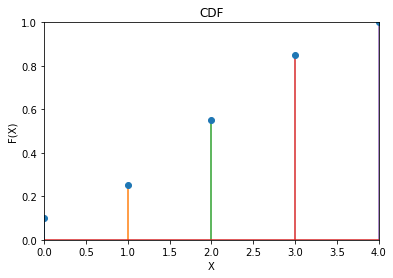
\includegraphics[width=10cm]{Assignment-1/Codes/Figures/CDF.png}
%     \caption*{Fig 1.1: Cumulative distribution function}
% \end{figure}

% \begin{figure}[h!]
%     \centering
%     \includegraphics[width=10cm]{Assignment-1/Codes/Figures/PDf.png}
%     \caption*{Fig 1.2: Probability density function}
% \end{figure}

% \subsection*{\boldsymbol{Problem\ 6.1.4}}
Find an expression for $F_A(x)$ using the definition. Plot this expression and compare with the result of problem 6.1.3
\subsection*{\boldsymbol{Solution}}\\
Given,
\begin{align}
A = \sqrt{V}
\end{align}

\begin{align} F_A(x) = P\ (\ A\ \leq\ x)\end{align}
\begin{align} F_A(x) = P\ (\ \sqrt{V}\ \leq\ x)\end{align}
\begin{align} F_A(x) = P\ (\ V\ \leq\ x^2)\end{align}
\begin{align} F_A(x) = F_V(x^2)\end{align}
From (6.1.2.1) we get\\

F_V(x)\ =\ \Bigg\{ 1\ -\ e^{-\alpha x}\ \ \ \ \ ;\ x \geq 0\\

Now\ for\ x^2,\ we\ substitute\ x^2\ in\ place\ of\ x\\

\begin{align}F_V(x^2) = \ \Bigg\{ 1\ -\ e^{-\alpha x^2}\ \ \ \ \ ;\ x^2 \geq 0\end{align}\\


\begin{align*}Putting\ \alpha\ =\ \dfrac{1}{2\sigma^2}\ =\ \dfrac{1}{2}\ \ \ [\because \ \sigma^2\ is\ given\ as\ 1]\end{align*}\\
We get,\\
\begin{align} F_V(x^2)\ =\ 1\ -\ e^\frac{-x^2}{2}\ \ \ \ ;\ x^2\ \geq\ 0\end{align}\\

\begin{mdframed}
Thus the CDF is derived as\\
\begin{align*} F_A(x) =  F_V(x^2)\ =\ 1\ -\ e^\frac{-x^2}{2}\ \ \ \ ;\ x^2\ \geq\ 0\end{align*}
The plot of this equation is shown in Fig 1.3.
\end{mdframed}
\begin{figure}[h!]
    \centering
    \includegraphics[width=10cm]{Assignment-1/Codes/Figures/cdf_actual_Vs_simulate.png}
    \caption*{Fig 1.3: CDF plot from derived equation}
\end{figure}
\subsection*{\boldsymbol{Problem\ 6.1.5}}
Find an expression for $p_A(x)$ using the definition.

\subsection*{\boldsymbol{Solution}}\\

The PDf can be derived by differentiating the CDF expression from the previous problem 6.1.4
\begin{align}f_A(x) = f_V(x^2)\end{align}
\begin{align}f_V(x^2) = \dfrac{d}{dx}(F_V(x^2))\end{align}
\begin{align}f_V(x^2) = \dfrac{d}{dx}(1 - e^\frac{-x^2}{2})\end{align}
\begin{align}f_V(x^2) = e^\frac{-x^2}{2}.x\end{align}
\begin{mdframed}
\begin{align*}p_A(x) = f_A(x) = e^\frac{-x^2}{2}.x\end{align*}
The plot of this equation is shown in Fig 1.4.
\end{mdframed}
\begin{figure}[h!]
    \centering
    \includegraphics[width=10cm]{Assignment-1/Codes/Figures/pdf_actual_Vs_simulate.png}
    \caption*{Fig 1.4: PDf plot from derived equation}
\end{figure}
\newpage
\text{The theoretical along with simulated PDf and CDF plot of 10,000 samples of Rayleigh random variables}
\newline 
\text{is shown in Fig 1.5 and Fig 1.6 -}

\begin{figure}[h!]
    \includegraphics[width=14cm]{Assignment-1/Codes/Figures/theo_Vs_sim_pdf.png}
    \caption*{Fig 1.5: Theoretical Vs Simulation PDf}
\end{figure}
\begin{figure}[h!]
    \includegraphics[width=14cm]{Assignment-1/Codes/Figures/theo_Vs_sim_cdf.png}
    \caption*{Fig 1.6: Theoretical Vs Simulation CDF}
\end{figure}
\end{document}
